%
% IFR
% $Id: ifr.tex,v 1.2 2006-05-15 13:19:58 alphonse.bendt Exp $
% 

Run--time  type information  in CORBA  is  managed by  the ORB's  {\it
Interface Repository}  (IR) component.  It allows  to request, inspect
and modify IDL  type information dynamically, e.g., to  find out which
operations an object supports. Some ORBs  may also need the IR to find
out whether  a given object's type  is a subtype of  another, but most
ORBs can do  without the IR by encoding this  kind of type information
in the helper classes generated by the IDL compiler.

In essence,  the IR is  just another remotely accessible  CORBA object
that offers  operations to retrieve  (and in theory also  modify) type
information.

\section{Type Information in the IR}

The  IR  manages  type   information  in  a  hierarchical  containment
structure that  corresponds to the structure of  scoping constructs in
IDL  specifications:   modules  contain  definitions   of  interfaces,
structures, constants  etc. Interfaces in turn  contain definitions of
exceptions, operations, attributes  and constants. Figure \ref{IR-fig}
illustrates this hierarchy.

\begin{figure}[htb]
  \begin{center}
    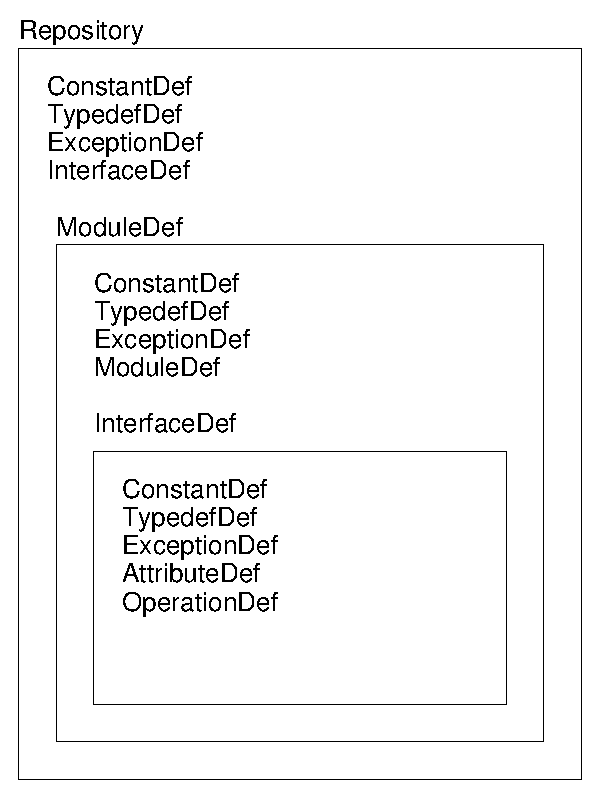
\includegraphics[width=5cm]{IFR/IR}
  \end{center}
\caption{Containers in the Interface Repository}
\label{IR-fig}
\end{figure}

The  descriptions  inside  the  IR  can  be  identified  in  different
ways. Every  element of  the repository has  a unique,  qualified name
which  corresponds  to  the  structure  of  name  scopes  in  the  IDL
specification. An interface {\tt  I1} which was declared inside module
{\tt M2} which in turn was  declared inside module {\tt M1} thus has a
qualified name  {\tt M1::M2::I1}. The  IR also provides  another, much
more   flexible   way   of    naming   IDL   constructs   using   {\it
Repository Id}s.  There   are  a   number  of  different   formats  for
RepositoryIds  but  every  Repository  must  be  able  to  handle  the
following format, which is marked  by the prefix {\tt "IDL:"} and also
carries  a  suffix   with  a  version  number,  as   in,  e.g.,  "{\tt
IDL:jacorb/demo/grid:1.0}". The name  component between the colons can
be set freely using the  IDL compiler directives {\tt \#pragma prefix}
and {\tt \#pragma ID}. If no such directive is used, it corresponds to
the qualified name as above.

\section{Repository Design}

When designing the  Interface Repository, our goal was  to exploit the
Java reflection  API's functionality to  avoid having to  implement an
additional data base for  IDL type descriptions. An alternative design
is to use the IR as a back-end to the IDL compiler, but we did not want
to  introduce such  a  dependency and  preferred  to a  have a  rather
``light--weight'' repository  server.  As  it turned out,  this design
was  possible because  the similarities  between the  Java  and CORBA
object models allow  us to derive the required  IDL information at run
time. As  a consequence,  we can  even do without  any IDL  at compile
time.  In addition  to this simplification, the main  advantage of our
approach lies in avoiding  redundant data and possible inconsistencies
between  persistent IDL descriptions  and their  Java representations,
because Java classes have to be generated and stored anyway.

Thus, the  Repository has to  load Java classes, interpret  them using
reflection  and   translate  them   into  the  appropriate   IDL  meta
information. To  this end, the  repository realizes a  reverse mapping
from   Java   to  IDL.   Figure   \ref{IR-Process}  illustrates   this
functionality,  where $f^{-1}$  denotes  the reverse  mapping, or  the
inverse of  the language  mapping.

\begin{figure}[htb]
  \begin{center}
    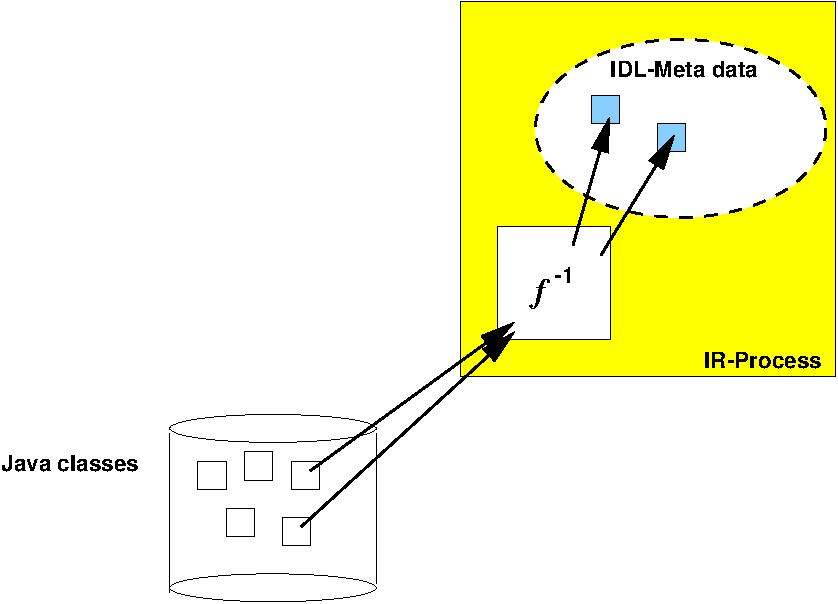
\includegraphics[width=7cm]{IFR/IR-Process}
\end{center}
\caption{The JacORB Interface Repository}
\label{IR-Process}
\end{figure}

\section{Using the IR}

For the ORB to be able to contact the IR, the IR server process must
be running. To start it, simply type the {\tt ir} command and provide
the required arguments:

\cmdline{ir /home/brose/classes /home/brose/public\_html/IR\_Ref}

The first  argument is  a path to  a directory containing  {\tt .class}
files and packages. The IR  loads these classes and tries to interpret
them as  IDL compiler--generated classes.  If it  succeeds, it creates
internal representations  of the  adequate IDL constructs. See below for
instructions on generating classes with IR information. The second
argument on  the command  line above  is simply the  name of  the file
where the IR stores its object reference for ORB bootstrapping.

To view the contents of the repository, you can use the GUI IRBrowser
tool or the query command. First, let's query the IR for a particular
repository ID. JacORB provides the command {\tt qir} (``query IR'')
for this purpose:

\cmdline{qir IDL:raccoon/test/cyberchair/Paper:1.0}

As result, the IR returns an InterfaceDef object, and {\tt qir} parses
this and prints out:

\begin{verbatim}
     interface Paper
     {
        void read(out string arg_0);
        raccoon::test::cyberchair::Review getReview(in long arg_0);
        raccoon::test::cyberchair::Review submitReview(
            in string arg_0, in long a rg_1);
        void listReviews(out string arg_0);
     };
\end{verbatim}

To start the IRBrowser, simply type

\cmdline{irbrowser [ -i <IOR-string> | -f <filename>]}

e.g.

\cmdline{irbrowser}

Note that if no arguments are supplied it will default to using
resolve\_initial\_references.

Figure \ref{fig:IRBrowser} gives a screen shot of the IR browser.

\bigskip
\begin{figure}[htb]
  \begin{center}
    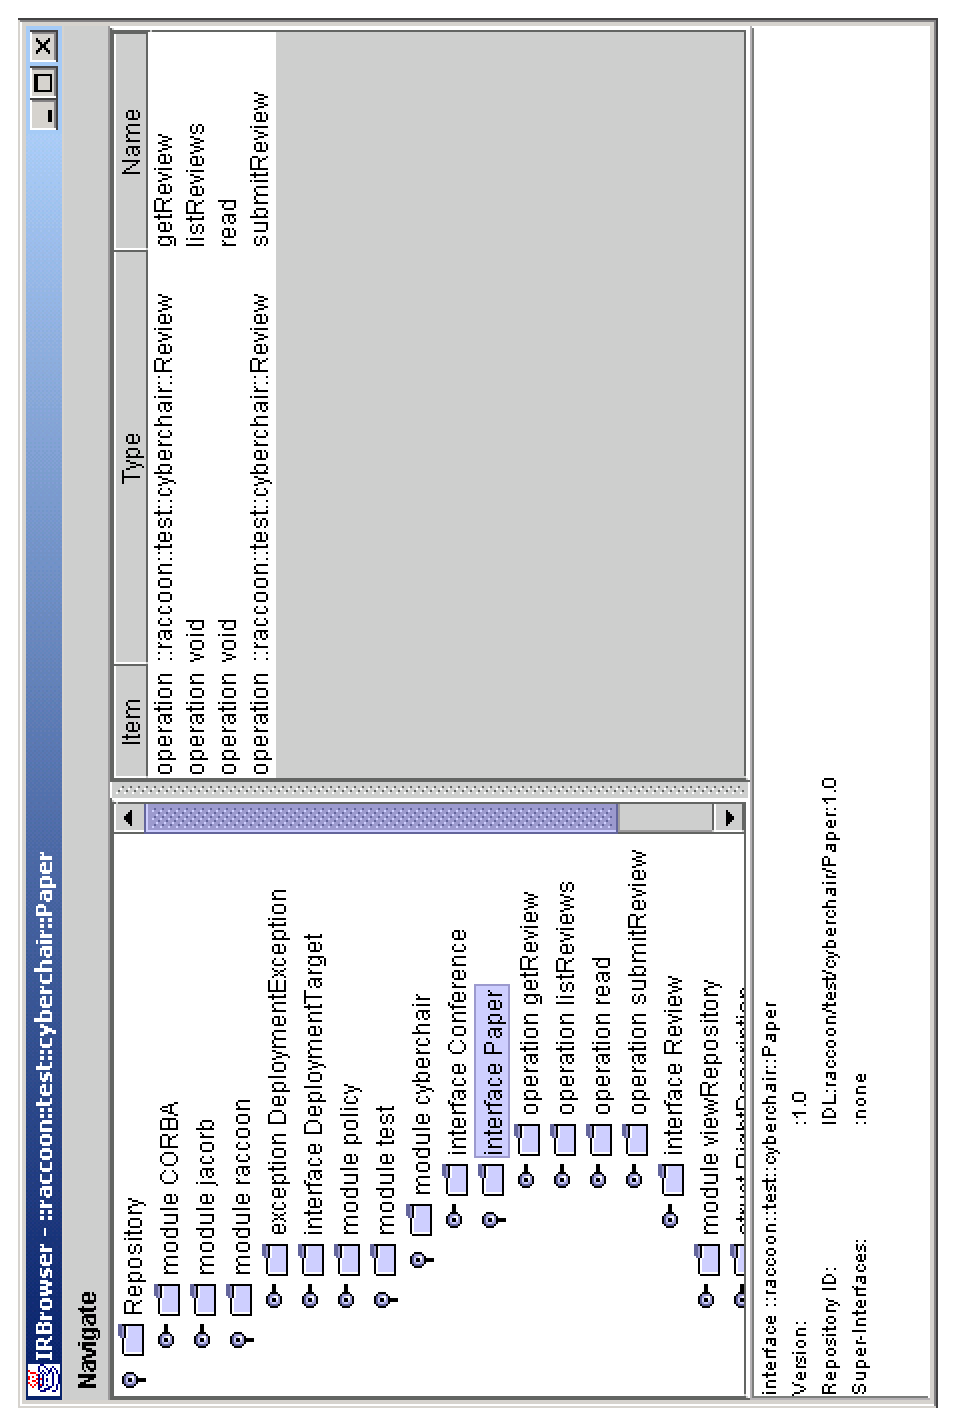
\includegraphics[width=11cm]{IFR/IRBrowser}
\end{center}
\caption{IRBrowser Screenshot}
\label{fig:IRBrowser}
\end{figure}

The Java classes generated by  the IDL compiler using the standard OMG
IDL/Java language mapping do not contain enough information to rebuild
all  of the  information contained  in  the original  IDL file.   For
example,  determining whether an  attribute in  an interface  was {\tt
readonly} or  not is not  possible, or telling the  difference between
{\tt  in}  and {\tt  inout}  parameter  passing  modes. Moreover,  IDL
modules are not  explicitly represented in Java, so  telling whether a
directory in  the class  path represents an  IDL module is  not easily
possible. For these  reasons, the JacORB IDL compiler  generates a few
additional  classes that hold  the required  extra information  if the
compiler switch {\tt -ir} is used when compiling IDL files:

\cmdline{idl -ir myIdlFile.idl}

The additional files generated by the compiler are:
\begin{itemize}
\item a {\tt \_XModule.java} class file for any IDL module X
\item a {\tt YIRHelper.java} class file for any interface Y.
\end{itemize}

\textbf{If no {\tt .class} files that  are compiled from  these extra
classes are found  in the class path passed  to the IR server  process,
the IR will not  be able  to derive any  representations.}
Note that  the IDL compiler does not make any non--compliant modifications
to any of the standard files that are defined in the Java language mapping
 --- there is only additional information.

One more caveat about these  extra classes: The compiler generates the
{\tt  \_XModule.java} class  only  for genuine  modules. Java  package
scopes created by applying the {\tt -d } switch to the IDL compiler do
not  represent   proper  modules  and   thus  do  not   generate  this
class. Thus, the contents of  these directories will not be considered
by the IR.

When an  object's client  calls the {\tt  get\_interface()} operation,
the ORB consults the IR  and returns an {\tt InterfaceDef} object that
describes the object's  interface. Using {\tt InterfaceDef} operations
on  this  description  object,  further  description  objects  can  be
obtained,  such as descriptions  for operations  or attributes  of the
interface under consideration.

The IR  can also be  called like any  other CORBA object  and provides
{\tt lookup()}  or {\tt lookup\_name()} operations to  clients so that
definitions can be searched for, given a qualified name. Moreover, the
complete contents of individual containers (modules or interfaces) can
be listed.

Interface   Repository  meta   objects  provide   further  description
operations. For a given {\tt  InterfaceDef} object, we can inspect the
different  meta   objects  contained   in  this  object   (e.g.,  {\tt
OperationDef} objects). It is  also possible to obtain descriptions in
form of a simple structure  of type {\tt InterfaceDescription} or {\tt
FullInterfaceDescription}. Since structures are  passed by value and a
{\tt   FullInterfaceDescription}    fully   provides   all   contained
descriptions,  no  further  ---possibly  remote  ---  invocations  are
necessary for searching the structure.


%%% Local Variables: 
%%% mode: latex
%%% TeX-master: "../ProgrammingGuide"
%%% End: 
